\documentclass[a4paper,12pt]{article}
\usepackage[a4paper]{geometry}
\geometry{top=1.0in, bottom=1.0in, left=0.1in, right=0.1in}
\setlength{\textwidth}{150mm}
\setlength{\oddsidemargin}{0.1cm}
\setlength{\evensidemargin}{0.1cm}
\setlength{\marginparsep}{0.1cm}
\setlength{\marginparwidth}{0.1cm}
\setlength{\marginparpush}{0.1cm}

\usepackage{minted}

%\usepackage[italian]{babel}
\usepackage{graphicx}
\usepackage[intlimits]{amsmath}
\usepackage{amsfonts}
\usepackage{listings}
\addtolength{\oddsidemargin}{-.0in}
\addtolength{\evensidemargin}{-.0in}

\usepackage{color}

\begin{document}

\begin{center}
 \huge \bfseries {Neilos}\\
 \normalfont \normalsize Version 1.4
\\[0.5cm]
\end{center}
\tableofcontents
\newpage
\section{Introduction}
Neilos is a content management system based almost completely on javascript. It is designed to be lightweight and fast and to use ajax for content loading. Furthermore, it is possible to use mysql, xml or both technologies to store content datas. Building a website with Neilos should be as simple as writing a basic xml file.
\section{Workflow of Neilos}
Neilos content and information consist and travel from the server to the client through entries. Entries can be stored in files or in a database, can have subentries or can load dinamically other entries.\\
The first thing Neilos does is loading resources/xml/config.xml, which is the main configuration of the site (it is an entry itself!). The main config usually (but not mandatory) loads the css styles, add the layout divs (see Structure section), and sets global variables, like default DOM target or default animation. \\
Finally, the main config loads other external entries, which can add articles, comments, html or php code through additional plugins.\\
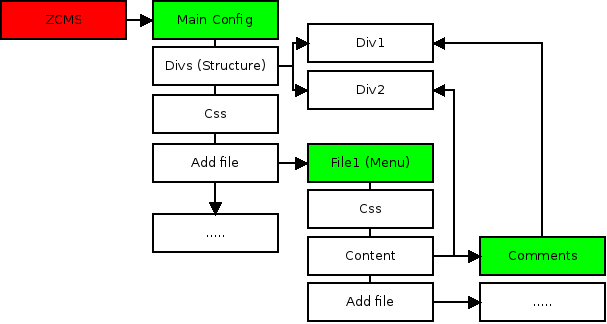
\includegraphics[scale=0.7]{Diagramma_neilos.png} \\
\subsection{Neilos Structure}
Nailos consists of 2 main blocks, the client-side javascript core (neilos.js) and the server-side php core (load.php).\\
Only the former is strictly necessary, the php core can be ignored in the simplest neilos configuration.\\
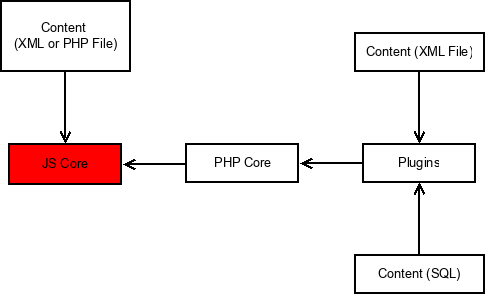
\includegraphics[scale=0.7]{neilos_structure.png} \\
\section{XML Entry Anatomy}
Every XML file is loaded with an $entryid$ parameter. Neilos searches for the entry with the id supplied.\\
An entry consists of 2 main sections: config and content. There can be also subentries, which are listed inside the parent entry and outside its config and content sections.\\
Content should consists of pure html, since it will be dumped to the DOM.\\
\footnotesize
\begin{minted}{xml}
<entry id='entryid'>
  <config>
    ...
  </config>
  <content>
    ...
  </content>

  <!-- Subentries -->
  <entry id='..'></entry>
  <entry id='..'></entry>
</entry>
\end{minted}
\normalsize
\subsection{DOM}
By default, every entry is added to the DOM with a main div ($\#id\_entry$) and 3 subdivs: .title, .content and .comments.\\
This behaviour can eventually be changed with some options (see below). If both title and content do not exist, the entry is not added to the DOM.
\subsection{Config}
The config tag is useful to load additionals css files, entries or to set useful settings.\\
Almost all options are inheritable to subentries. Available options are:
\begin{list}{-}{}
\item \begin{minted}{xml}
<pagetitle>       
      \end{minted}
Change the title of the page
\item \begin{minted}{xml}
<title>       
      \end{minted}
Set the title of the entry
\item \begin{minted}{xml}
<css id='css_id'>       
      \end{minted}
Load an external css file. The id is used to identify the css in order to remove or replace it afterwards.
\item \begin{minted}{xml}
<author>m3l7</author>
<date>2011-09-08</date>
      \end{minted}
Specify the date and author of the entry. They will be added to the DOM in the .title before everything else.
\item \begin{minted}{xml}
<structure_div overwrite='false' parent="#parent">div_name</structure_div>       
      \end{minted}
Add a div to the DOM. (See Structure section)
\item \begin{minted}{xml}
<target>target</target>       
      \end{minted}
specify where the entry should be added in the DOM (jquery selector).
\item \begin{minted}{xml}
<animation speed='fast' speedshow='normal' speedhide='slow'
 type='fade/slide/hide'>enabled</animation>
      \end{minted}
Select the type and speed of the animation. If speedshow/speedhide is set, it will be used instead of speed for showing/hiding the entry.
The speed can have the format $\#n$, where n is the animation time in milliseconds.
\item \begin{minted}{xml}
<home>#home.xml</home>
      \end{minted}
Set the default home page. See links section for informations about links meaning.
\item \begin{minted}{xml}
<display entries="showfirst/show/hide"></display>
\end{minted}
Choose if content (and comments) should be visible or not. If showfirst is set, the entry is visible only if it's the first child.\\
Default: show
\item \begin{minted}{xml}
<load_file mode='loadwhenshown' 
entryid="menu">resources/xml/menu.xml</load_file>
      \end{minted}
Load an external file. Neilos will add the content inside the jquery selector tag.\\
If mode='loadwhenshown' is set, the file is loaded only when the entry is toggled.
\item \begin{minted}{xml}
<clear>false</clear>
\end{minted}
If true, the target will be cleared before adding the entry.
\item \begin{minted}{xml}
<visibiity>true</visibility>
\end{minted}
If true, the entry will not be shown.
\item \begin{minted}{xml}
<skipsubentries>true</skipsubentries>
\end{minted}
If true, subentries will be ignored.
\item \begin{minted}{xml}
<type>notitle</type>
\end{minted}
If set, title will be ignored.
\item \begin{minted}{xml}
<default_extension>xml</default_extension>
\end{minted}
Set the default extension of content files. Can be xml or php and can be set only in the main config (config.xml)\\
Neilos will cycle throigh the other extensions automatically if the file is not found.
\item \begin{minted}{xml}
<class>optionalclass</class>
\end{minted}
Add an additional class to the entry.
\item \begin{minted}{xml}
<click prevent_default='true' updateurl='true' href='filename' remove='true'></click>
\end{minted}
Open an internal link (specified by href) when the entry is clicked. If prevent\_default is set, the normal toggle behaviour is avoided.If updateurl is set true, the url bar will be updated to the href link.\\
If remove is set, the entry is removed after being clicked.
\item \begin{minted}{xml}
<alias source='page' file='filename.php'></alias>
\end{minted}
Open filename.php when \#page link is requested
\item \begin{minted}{xml}
<tag>tag1,tag2</tag>
\end{minted}
Attach a tag to the entry. Tags are useful to load dinamically only certain "categories" of entries. Currently, tags are only supported when using the php core.
\item \begin{minted}{xml}
<plugin></plugin>
\end{minted}
Add a plugin to the entry. See the proper section.
\item \begin{minted}{xml}
<updateurl>#!url</updateurl>
\end{minted}
Update the url bar to the specified url.
\item \begin{minted}{xml}
<delete delay='2000' id='id'></delete>
\end{minted}
Delete the specified entry. Wait 2000ms before deleting.
\item \begin{minted}{xml}
<checkform selector='#form' href='#!link'/>
\end{minted}
Check the specified form, and pass its input boxes with check='true' property to href as an additional parameter ($\&param1='input'$).\\
This is only a proof of concept. Should be extended in the future.
\end{list}
\normalsize
\subsection{Link to entries}
It is possible to specify just the name of the file in which the entry is stored. In this case the php core will not be used. 
\begin{minted}{xml}
 <load_file entryid="menu">
 resources/xml/menu.xml</load_file>
\end{minted}
To use the php core, use this syntax:
\begin{minted}{xml}
 <load_file entryid="menu"> resources/load.php?data="filename"
 &id="menu"&tag="tag"&sql="true"&file="false"</load_file>
\end{minted}
The data tag is the XML filename where the entry is stored. If a database is used for storage, data will be ignored or will be used as id if id parameter is not set.\\
sql and file parameters are used to override the default behaviour
\subsection{Menu links}
A typical menu link points to index.php\#!page.xml \ .Neilos will load automatically page.xml and will add it to the site with ajax, using the file name as id. The file must be located in resources/content/.\\
If the file is not found and no extension is provided, Neilos will try to add .xml and .php extensions to the file name.\\
When using the php core, it is possible to use these simplified syntax:
\begin{minted}{xml}
 index.php#!load.php?parameters
\end{minted}
instead of 
\begin{minted}{xml}
 index.php#!resources/load.php?parameters
\end{minted}
and
\begin{minted}{xml}
 index.php#!load/home?parameters
\end{minted}
instead of
\begin{minted}{xml}
 index.php#!resources/load.php?data="home"&parameters
\end{minted}



\section{Variables}
\subsection{Server (PHP Core) variables}
Server variables are stored in vars.php

\begin{list}{-}{}
\item \begin{minted}{xml}
$_SITENAME = 'n';
\end{minted}
Name of the site. Mandatory.
\item \begin{minted}{xml}
$_ANALYTICS = FALSE;
$_ANALYTICS_ID = 'xxx';
$_STATCOUNTER = FALSE;
$_STATCOUNTER_PROJ = 'xxx';
$_STATCOUNTER_SEC = 'xxx';
\end{minted}
Stat counter and Google Analytics parameters.
\item \begin{minted}{xml}
$_SITENAME = 'n';
\end{minted}
\item \begin{minted}{xml}
$_DEFAULT_STORAGE = 'sql';
$_DEFAULT_STORAGE = 'file';
\end{minted}
Select the default storage.
\item \begin{minted}{xml}
$_SQL_HOST = "xxx";
$_SQL_USER = "xxx";
$_SQL_PASS = "xxx";
$_SQL_DB = "xxx";
\end{minted}
MySQL parameters.
\end{list}


\subsection{Client (JS Core) variables}
Neilos has an internal parser which substitutes some special strings inside content entries. At this stage, it's very limited.
\begin{list}{-}{}
\item \begin{minted}{javascript}
$_version
\end{minted}
show Neilos version
\end{list}
\normalsize
\section{Structure}
Structure objects can be created using the following methods:
\subsection{js methods}
\begin{list}{-}{}
 \item Neilos.Structure.new\_div: this will create a simple div. Additional classes can be added.
\item Neilos.Structure.new\_tab: this will create an entry (\bfseries{TODO} \normalfont Rename to new\_entry?). An entry is a div with 2 or 3 subdivs: [title], content, comments. Each subdivs has 2 subdivs: \_text and \_text\_right
\end{list}
\subsection{xml methods}
\begin{list}{-}{}
  \item \begin{minted}{xml}
<structure_div overwrite='false' parent="#parent">         
        \end{minted}
create a div and a subdiv \_content. It is created at the end of the current DOM (or inside parent, if specified), so it should be used only in the main config. It must be placed inside $<$config$>$ tag.
  \item \begin{minted}{xml}
<structure_tab parent="#parent">         
        \end{minted}
create a standard container for an entry
\end{list}

\section{SEO}
Starting from version 1.2.2, Neilos can be indicized by Google, using the standard \_escaped\_fragment method.\\
A $fallback\_load.php$ and a modified index.php are provided, which can load the site using php only code.
At the moment, $fallback\_load.php$ loads all the content, but generally not in the correct order and with the correct containers; for this readon it is not suitable for every day use as a replacement for the default js code.

\section{Plugins}
Starting from version 1.3, Neilos supports a server side plugin architecture.\\
To load a plugin, just add the "plugin" tag to the config section, i.e.
\begin{minted}{xml}
    <plugin>
	    <load plugin="More">
                <param name="entries_per_page">1</param>
                <param name="show_more">1</param>
            </load>
    </plugin>
        \end{minted}
Dev Version supports a basic client side plugin architecture. To load a js (client side) plugin, use
\begin{minted}{xml}
 <plugin type='js'>name</plugin>
\end{minted}

\subsection{List of plugins}
\subsubsection{More (Server)}
More plugin prevents neilos to load all subentries of a given entry if they are too many.\\
It is possible to specify how many subentries have to be shown at the same time, and choose to show a more button for showing the next page.\\
\bfseries Parameters:\\
\normalfont \normalsize -entries\_per\_page: number of entries to display in a single 'page'.\\
-show\_more: if set to 1, a button which loads the next page will be visible.\\
\subsubsection{Loader (Server)}
Load entries and add them as subentries using the php core. This is different from the standard $load\_file$ situation where the entries are loaded separately by the js core.\\
This is useful when additional entries have to be loaded as subentries, i.e. to be postprocessed by other plugins.\\
\bfseries Parameters:\\
\normalfont \normalsize Same as the standard $load\_file$ GET parameters of the php core. (i.e. data,tag,sql,file)
\section{Admininstration}
Starting from 1.4, Neilos has a very poor admin interface. At the moment, it's only possible to convert all the content xml files to the database and back, and to clean the database. There is no support for login or multiuser, so it's not safe to publish the admin/ folder.
\end{document}
